%!TEX root = main.tex
\section{Assemblage d'objets 3D sur le web avec architecture évènementielle}
\label{sec:us}
L'expérimentation propose de répliquer une collaboration réaliste entre différents 
participants travaillant à distance. Ce cas d'étude présenté dans 
\cite{Desprat2017} souligne plusieurs aspects relatif à la fiabilité du modèle et de 
son implantation de deux manières: 
\begin{itemize}
	\item fonctionnelle : manipulation et visualisation 
	3D, historique ;
	\item et technique : récupération de l'information, cohérence des 
	données, disponibilité du réseau.
\end{itemize}

Quant à l'observation du comportement des participants, elle est 
effectuée de manière quantitative (\textit{monitoring}) et de manière qualitative 
(questionnaire) lors de l'exécution d'une tâche coopérative au sein de l'application.

%The 3D data issued from X (cite) represent the different parts of a 3D printed 
%case for a camera based on RaspberryPi and a Thermal Printer. Data used in 
%the 
%experiment are triangulated surfaces converted from the STL files given. The 
%case 
%is composed of N connected components. (see figure F).
\paragraph{Tâche à effectuer}
Les participants devaient assembler les différentes parties d'un modèle 3D en 
utilisant l'application 3DEvent et les fonctionnalités décrites précédemment 
\info{ref section foncitonnalités} pour que le résultat corresponde à l'assemblage 
donné en exemple (images). La complexité de la tâche a été modulée selon 
plusieurs facteurs : le nombre de parties composant le modèle et le nombre de 
collaborateurs. Afin de permettre la manipulation des objets 3D facile à 
apprendre et utiliser, il a été choisi de conserver des manipulations de haut niveau.
%Participants had to assemble in a web-browser the different parts of a model 
%using 3DEvent application and features described in Section \ref{sec:ui} to 
%match 
%a final given assembly. The complexity of the task was modulated by the 
%number 
%of parts composing the assembly and the number of collaborators. We wanted to 
%keep the 3D manipulation tasks at high level to be easy to learn/use.
\paragraph{Population}
L'expérience a été conduite sur 12 groupes de deux ou trois participants chacun. 
Chaque participant était localisé en France dans une zone urbaine avec de bonnes 
infrastructures en travaillant sur des réseaux distincts avec une bonne connexion 
internet (au moins 20Mb/s) pour éviter d'avoir des latences extrêmes (>10 
secondes) au cours 
des expérimentations. Les participants étaient des étudiants de Master ou de 
Doctorat en informatique (pas nécessairement familiers avec les environnements 
3D). Les participants étaient autorisés à communiquer entre eux par chat.


\paragraph{Procédure}
Les modèles utilisés lors de l'expériences sont décrits dans le Tableau 
\ref{table:summary}. L'expérimentation se déroule en trois phases : 
\begin{description}
	\item[Phase d'essai] Chaque participant s'entraîne pendant 5-10 minutes sur un 
	modèle de test dans l'application pour se familiariser avec l'interface et les 
	fonctionnalités proposées.
	\item[Phase solo] Le participant effectue un assemblage du modèle Rotor ou 
	Camera Box.
	\item[Phase de collaboration] Un groupe de participants réalise deux 
	assemblages sur 
	\begin{enumerate*}[label=(\roman*)]
		\item un petit modèle (10 ou 12 parties) puis
		\item un plus gros modèle (16 parties).
	\end{enumerate*}
	La phase de collaboration a été répétée six fois : trois fois 
	avec un groupe de deux participants et trois fois avec un groupe de trois 
	participants.
\end{description}

Du fait que les participants pouvaient participer à différentes configurations de 
groupe durant la phase de collaboration, plusieurs modèles 3D avec des 
caractéristiques similaires (nombre de parties et nombre de triangles) ont été 
présentés pour éviter les biais liés à l'apprentissage.

\begin{table}[ht]
	\centering
	\caption{Modèles utilisés durant l'expérimentation}
	\label{table:summary}
	\begin{tabular}{cccc}\hline
		\textbf{Modèle}  & \textbf{Nombre de parties} &  \textbf{Nombre de triangles} 
		& \textbf{Taille totale}  \\ \hline
		Rotor      &   10  &    62k & 4Mo        \\
		Camera box        &   12  &    67k & 5Mo        \\
		Car      &   16  &      170k & 8Mo \\       
		Living room      &   16  &      200k & 9Mo \\    \bottomrule
	\end{tabular}
\end{table}
\paragraph{Initialisation}

Pour chaque phase, l'application a été initialisée par le chargement des parties du 
modèle dans la bibliothèque d'objets chez chaque participant. Les parties des 
objets ont volontairement été positionnés (rotation et homothétie) aléatoirement 
afin que les utilisateurs aient à manipuler les différentes fonctionnalités. Cette 
configuration nous permet d'observer l'activité à l'intérieur de chaque groupe durant 
l'expérimentation. Chaque participant a reçu une image de l'assemblage à réaliser 
(la tâche à compléter). 

\paragraph{Données collectées}
Pour chaque expérimentation et chaque participant, le temps de complètement, le 
nombre d'évènements générés et l'horodatage de chaque évènement pour 
observer le complètement de la tâche en termes de vitesse et d'efficacité ainsi 
que les effets sur le temps d'implication d'un collaborateur selon le nombre de 
collaborateurs. 

L'enregistrement des données commence lorsque le premier évènement sur la 
scène initialisée est généré (horodatage du premier évènement); et il s'arrête 
lorsque le groupe indique que la tâche à compléter est terminée (horodatage du 
dernier évènement est considéré).


\paragraph{Questionnaire}
En dehors des données collectées, les participants à devaient remplir un 
questionnaire basé sur l'expérimentation pour exprimer leurs retours qualitatifs 
concernant leur expérience (Annexe \ref{app:quest}) \info{ajout questionnaire}. 

Le questionnaire est inspiré de \cite{Lewis1995}, qui permet d'évaluer la facilité 
d'utilisation du système et l'implication dans la collaboration de chacun des 
participants. En utilisant une échelle de notation sur sept points \cite{Lewis1993}, 
(1~:~pas d'accord~; 7~:~d'accord) pour avoir assez de points de discrimination.



Au cours des différentes sessions collaboratives, l'application à produit plusieurs 
centaines d'évènements (environ 300 par session). Les expérimentations ont été 
réalisées sur plusieurs dispositifs notamment un \textit{smartphone} avec une 
connexion 4G. 
La Figure \ref{fig:screenshots} montre quelques captures d'écran durant une 
session collaborative sur le modèle Rotor ; et la Figure \ref{fig:ui4} montre les 
premiers évènements enregistrés dans la base de données\info{mettre ailleurs?}. 
Les boîtes englobantes représentent la sélection des différents collaborateurs 
pendant la session.
\begin{figure}[ht]
	\centering
	
	\subfloat[Translation (environnement 3D) et visualisation de l'historique 
	(panneau 
	latéral)]{\includegraphics[width=0.7\textwidth]{eps/1translatehisto.eps}\label{fig:ui1}}\hfill
	\subfloat[Rotation (environnement 3D) et outils pour la manipulation d'objet 3D 
	(panneau 
	latéral)]{\includegraphics[width=0.7\textwidth]{eps/2rotatedetail.eps}\label{fig:ui2}}\hfill
	\subfloat[Mise à l'échelle (environnement 3D) et liste des collaborateurs 
	(panneau 
	latéral)]{\includegraphics[width=0.7\textwidth]{eps/3scalecollab.eps}\label{fig:ui3}}\hfill
	\caption{Interface utilisateur pendant une session collaborative (trois personnes)}
	\label{fig:screenshots}
\end{figure}

\begin{figure}[ht]
	\centering
	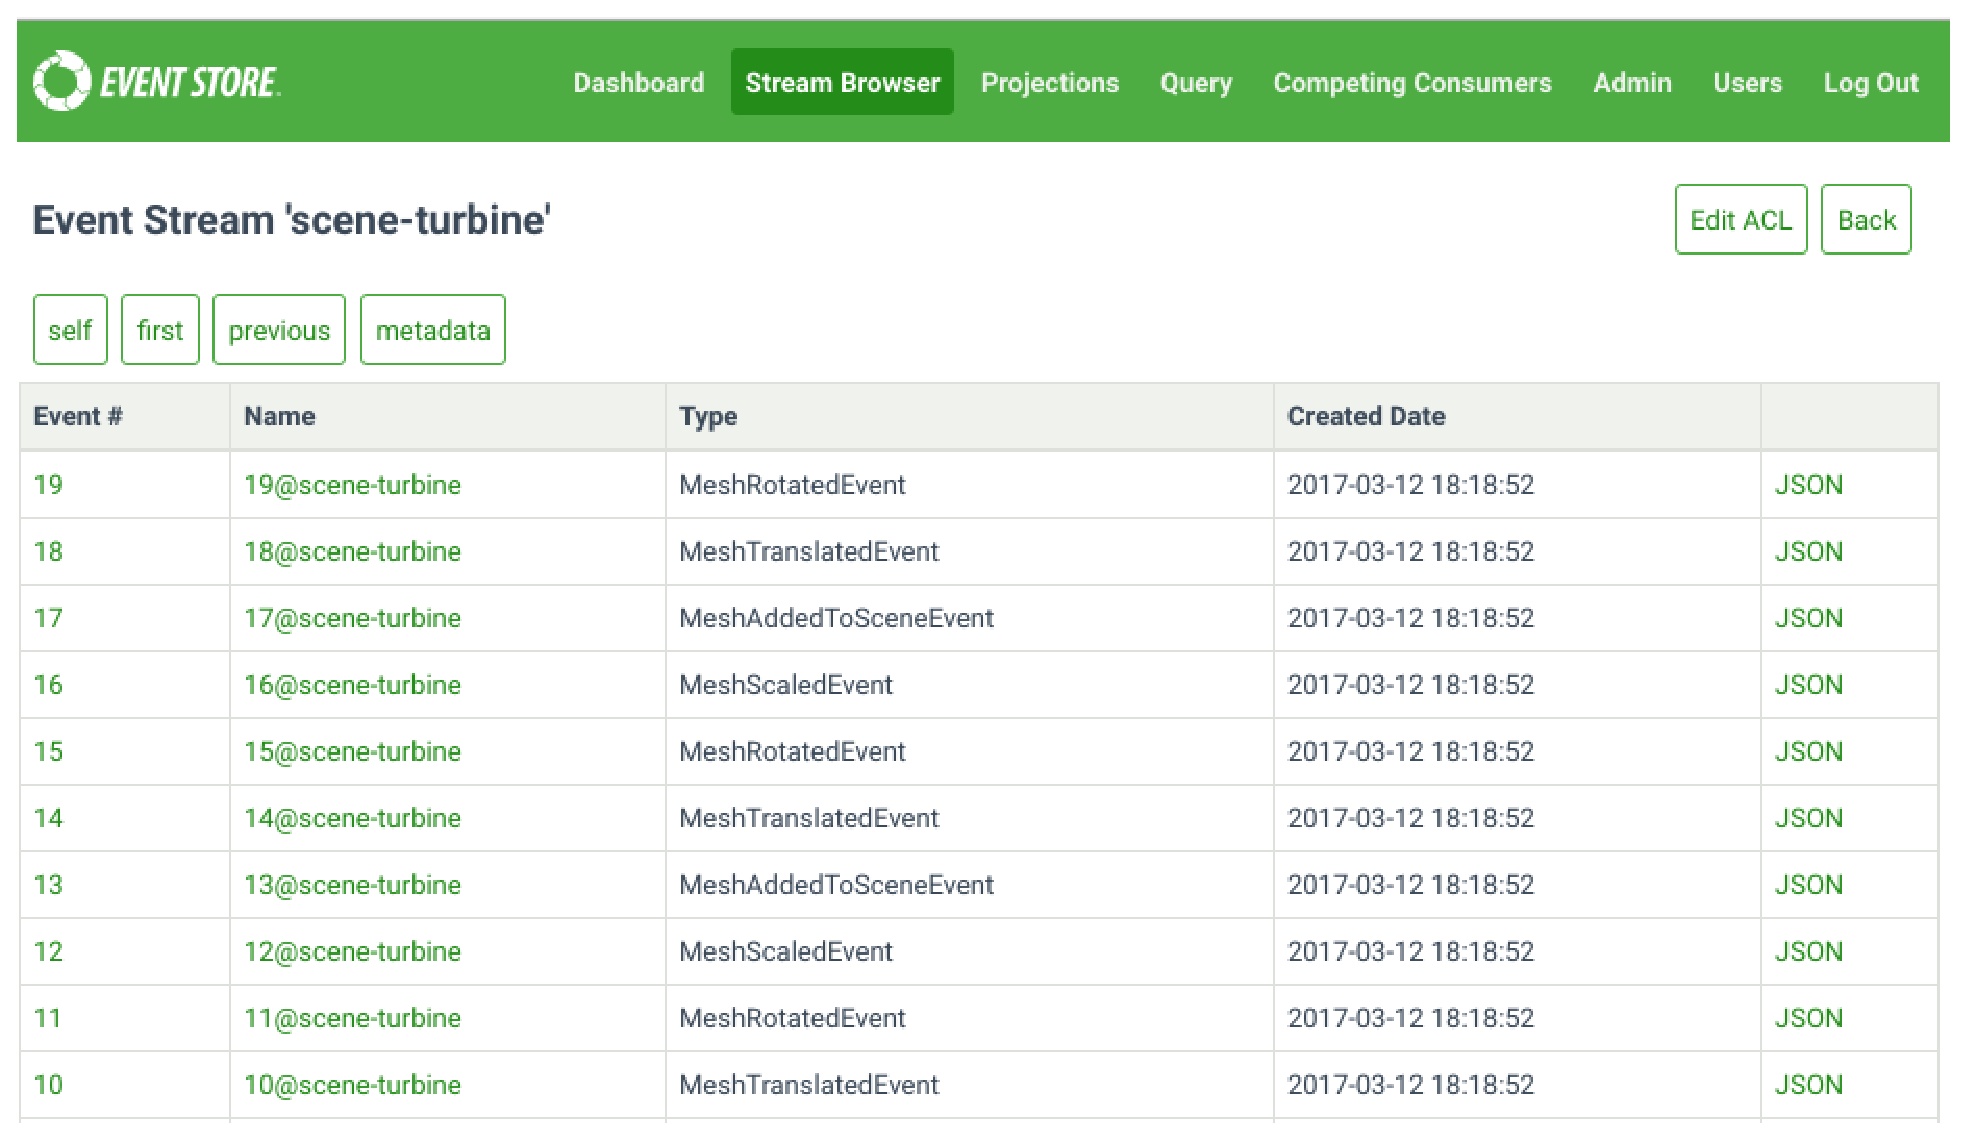
\includegraphics[width=\textwidth]{eps/eventstore.eps}
	\caption{Persistance long-terme (Event Store\textsuperscript{\textregistered}), 
		base de données/outil de monitoring}
	\label{fig:ui4}
\end{figure}

\subsection{Résultats et Discussion}
\label{sec:res}


\paragraph{Analyse des interactions}
Les traces des utilisateurs récupérées au cours des expérimentations sont la base 
du travail d'analyse qui est présenté ici. Ces traces, composées d'évènements 
générés par les utilisateurs, permettre de savoir qui (Figure \ref{petita}) a fait quoi 
(Figure \ref{petitb}) lors des sessions collaborative. Généralement, le \og qui\fg{} 
est assez facile à retrouver lors de la récupération des traces. Le \og quoi\fg{} 
cependant nécessite que les notifications aient une signification précise et proche 
du métier. Grâce au travail de découpage et de dénomination des évènements 
effectué en amont, le journal d'évènements (\textit{log}) indique précisément tout 
ce 
qui s'est passé lors de la session d'un point de vu métier. Cette fonctionnalité est 
intéressante dans le contexte de la traçabilité des données et lors d'audits sur 
l'assemblage. 

Figure \ref{fig:collabsession} montre deux angles d'enregistrement d'une session 
sur le modèle \textit{living room}. Au début de la session, beaucoup d'objets sont 
ajoutés (meshAddedToSceneEvent). Seul un utilisateur a ajouté un objet en 
utilisant la fonctionnalité pour déposer un objet à un endroit spécifique de la scène 
(meshDropped \info{name it}). Le nombre d'évènements concernant la sélection et 
la désélection est à peu près similaire aux exception. La différence s'explique par 
le fait que l'évènement de désélection n'est pas déclenché lors d'un changement 
d'objet sélectionné, car la désélection n'est pas effectuée explicitement par 
l'utilisateur. Au commencement, les participants ont fortement interagit (jusqu'à 20 
évènements en 15 secondes). Cela s'explique par le recours massif à l'ajout 
d'objets dans la scène pour composer le modèle et la mise à l'échelle de ceux-ci 
(du au positionnement arbitraire des objets de la bibliothèque). Ensuite, les trois 
utilisateurs interagissent ensemble durant quelques minutes avant que l'un d'entre 
eux ne quitte et ne reviennent quelques secondes plus tard (informations 
récupérées à partir du journal d'évènements lié aux agrégats utilisateurs). Enfin, le 
nombre d'évènements diminue montrant la fin de l'activité, les utilisateurs finissant 
la tâche et ajustant les derniers objets.

L'implication d'un utilisateur peut être vue par le prisme de la fréquence de ses 
contributions et la variété de fonctionnalités utilisées, autrement dit, les différents 
types d'évènement produits. L'analyse d'une session apporte plusieurs indicateurs 
tout au long de la session. Par exemple, l'absence d'un utilisateur pendant une 
longue période peut indiquer une déconnexion. Ou encore, l'utilisation trop 
fréquente d'un type d'évènement (ou d'un motif d'évènements répété) peut montrer 
une faiblesse de l'ergonomie de l'interface. Pour ce dernier aspect, on peut prendre 
l'exemple dans la Figure \ref{petitb} à 45s, on remarque un nombre élevé de 
MeshScaledEvent. A posteriori, nous nous sommes rendu compte que la 
fonctionnalité était mal calibrée pour l'échelle du modèle et nécessitait donc de s'y 
reprendre à de nombreuse fois pour réaliser la bonne transformation.

\begin{figure}[ht]
	\centering
	
	\subfloat[Par 
	utilisateur]{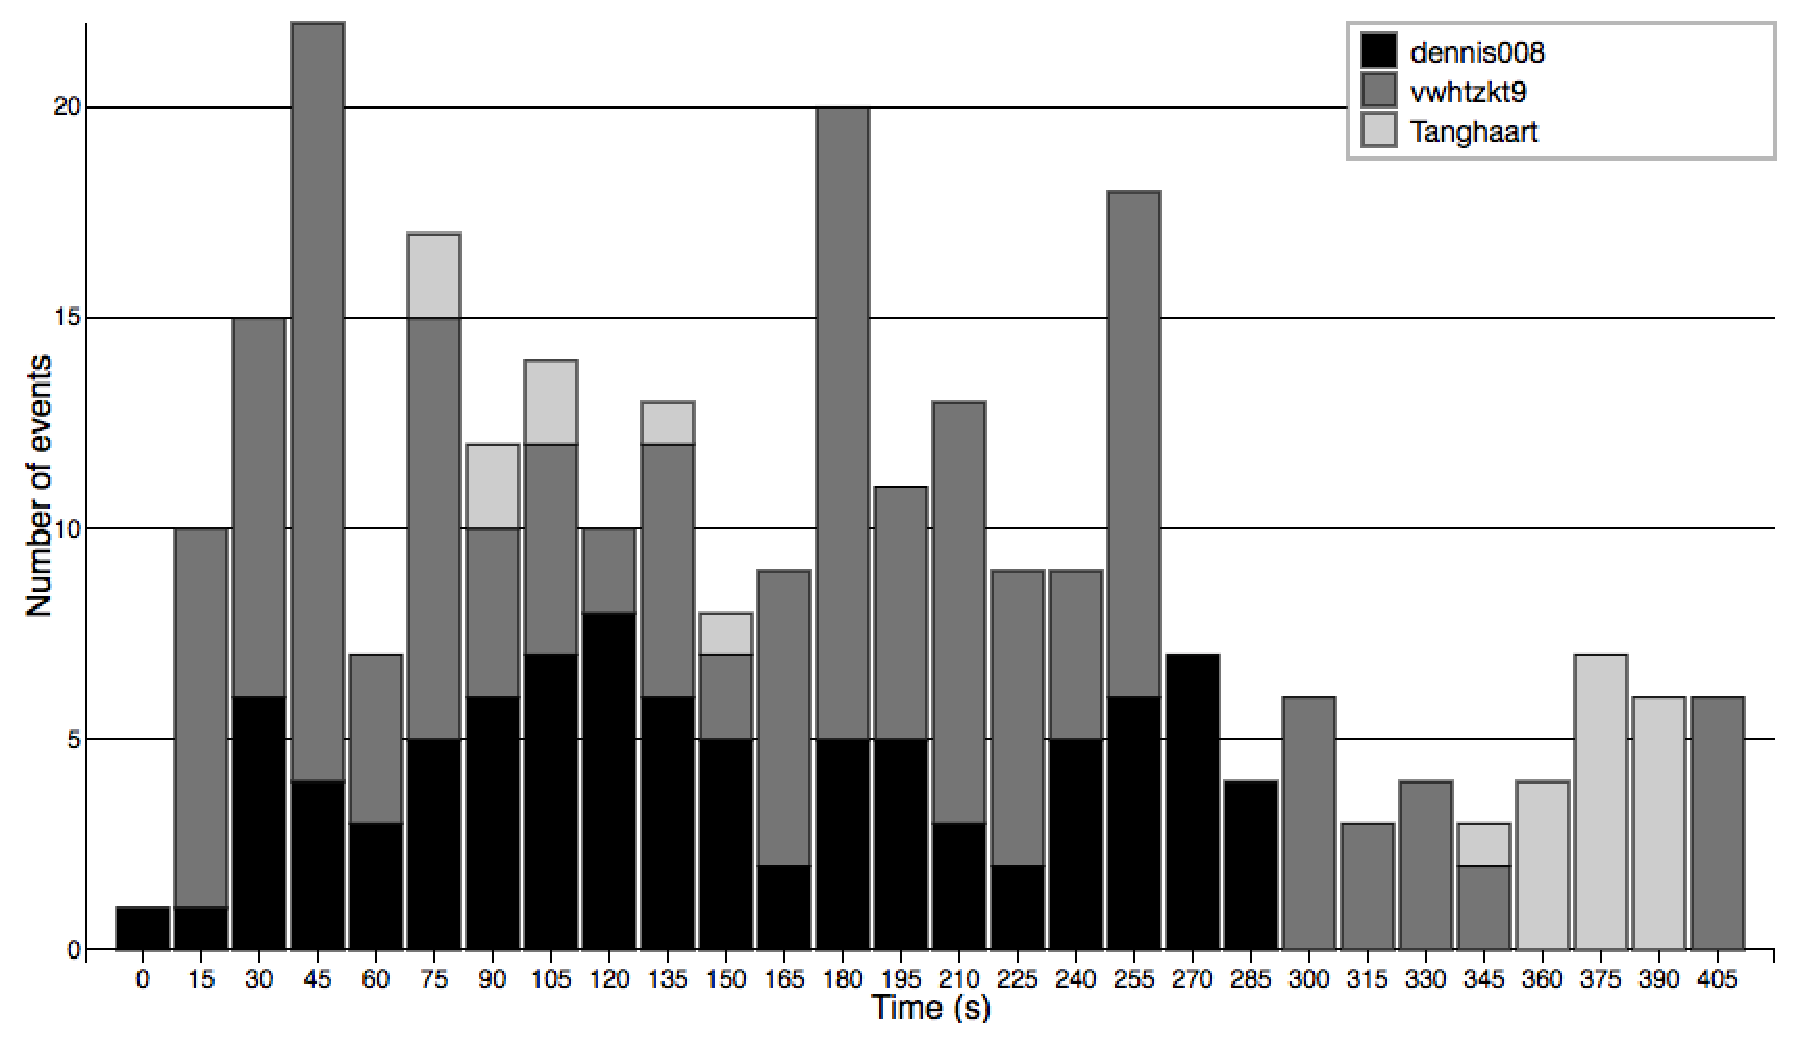
\includegraphics[width=\columnwidth]{eps/byuser.eps}\label{petita}} \\
	\subfloat[Par type 
	d'évènement]{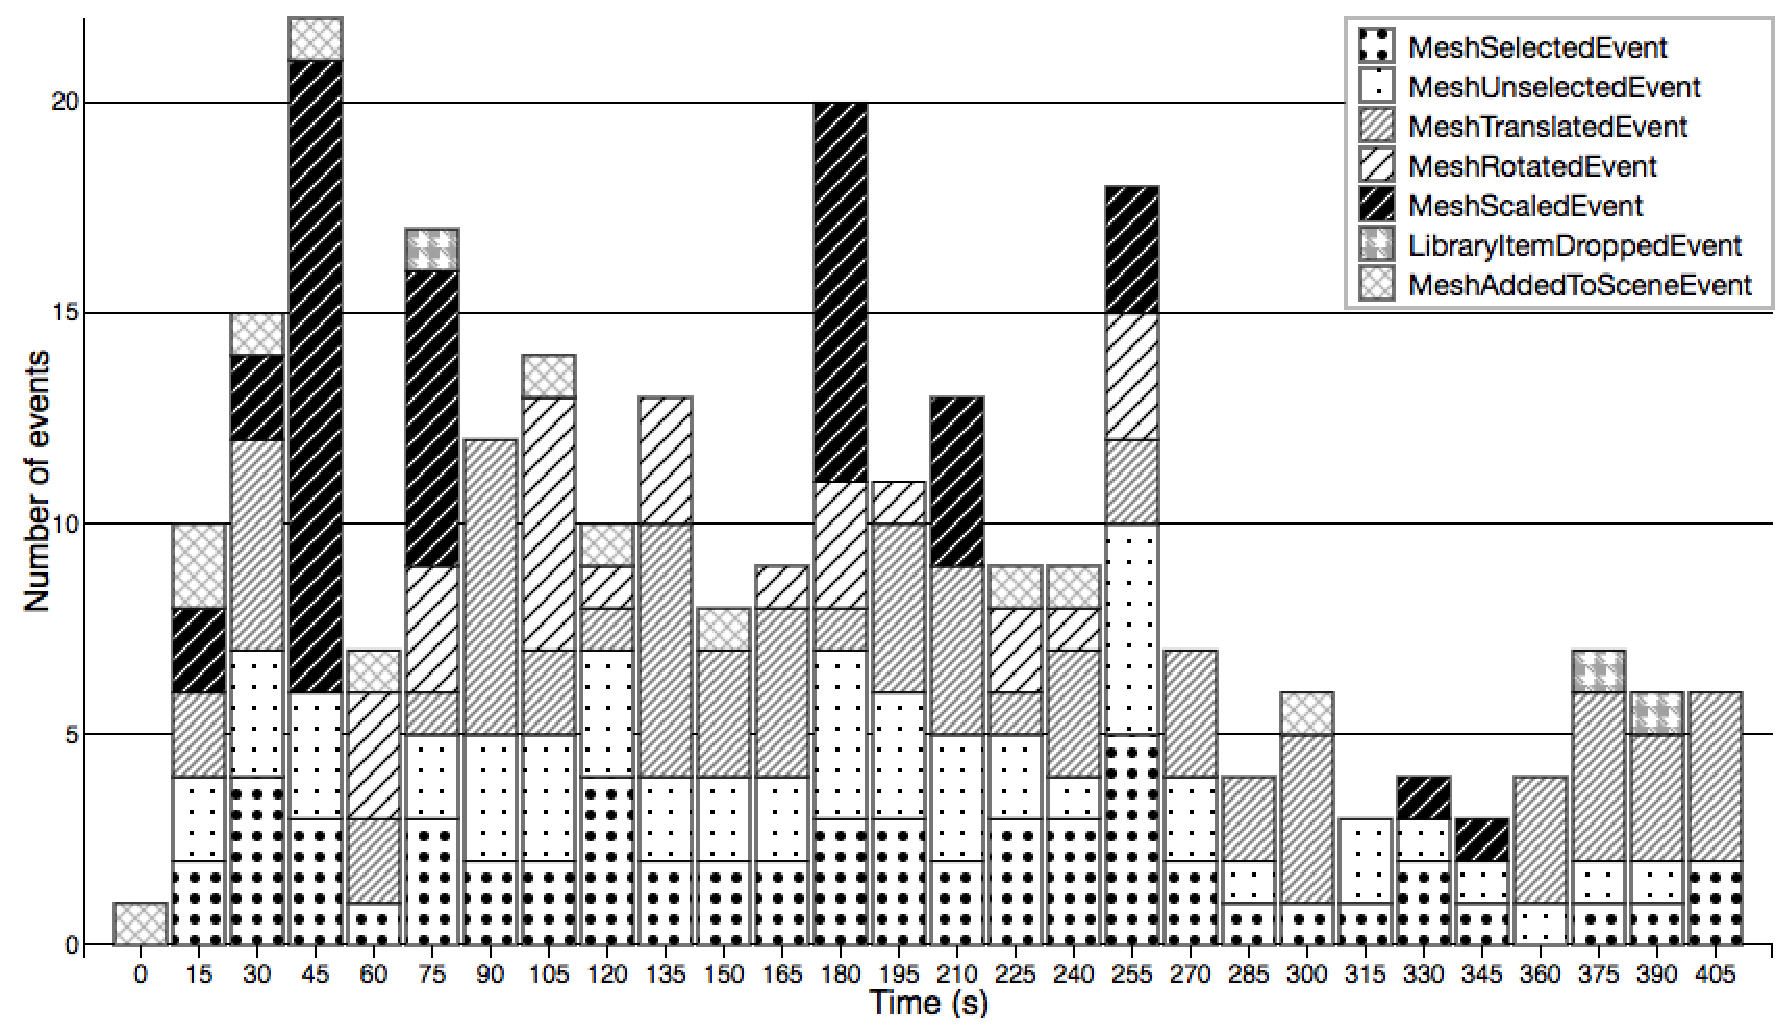
\includegraphics[width=\columnwidth]{eps/byevents.eps}\label{petitb}}
	\caption{Résumé d'une session collaborative au cours du temps}
	\label{fig:collabsession}
\end{figure}

\paragraph{Questionnaires}
Après chaque expérimentation, le participant a rempli directement un questionnaire 
à propos des phases solo et collaboratives qu'il a effectuées via le formulaire en 
ligne. les résultats obtenus sont compilés dans la Figure 
\ref{fig:questionnaire} sous la forme de boîte à moustache. Cette représentation 
est un moyen rapide de figurer le profil essentiel des résultats des mesures 
quantitatives effectuées.
Globalement, les tâches ont été réalisées plus rapidement et plus efficacement 
de manière collaboration que de manière solo. La facilité d'utilisation et la 
simplicité de l'interface sont également soulignées positivement par plusieurs 
utilisateurs. Comme indiqué dans les retours d'expérience négatifs, la stabilité du 
réseau a parfois amené un peu de frustration chez certains participants. 
Cependant, les participants ont trouvé que la cohérence de l'environnement lors de 
la collaboration et la récupération des données était plus qu'acceptable. Cette 
remarque s'accompagne également du fait que la distribution des données s'est 
effectuée correctement\info{proove it}, leur permettant de coopérer efficacement.

Durant l'une des expérimentations en phase collaborative, nous avons eu un 
participant avec une latence de plus de 10s à certains moment, mais malgré cela, 
le groupe nous a notifié que cela n'avait pas affecté la collaboration. Au long des 
expérimentations, quelques conflits ont été levés sur différentes opérations à 
différent niveaux. Au niveau réseau (mauvaise version, désynchronisation), la 
politique en place est d'annuler l'évènement et de resynchroniser les utilisateurs 
entre eux. Au niveau des utilisateurs (opérations opposées sur le même objet), la 
résolution du conflit doit passer par un canal externe (chat) pour que les 
utilisateurs se mettent d'accord.  

%During one of the experiments, we had a latency of 10 seconds, but despite it, 
%participants said that the latency did not affect the collaboration. Few conflicts 
%were raised (multiple selection of the same item) but rapidly solved through chat 
%communication. 

Dans toutes les expérimentations menées, le but a été atteint dans pratiquement 
le même temps (10-15 minutes). La facilité d'utilisation du système n'est donc pas 
en reste malgré quelques aspects à améliorer. Rappelons que bien que la 
complexité des modèles ne soit pas extrême, tous les participants étaient 
débutants sur le système et n'était pas forcément familier de ce genre 
d'application. 
Le fait que l'application soit basée web à également joué en faveur de 
l'appropriation de l'application car il a semblé assez naturel aux participants de se 
rendre à l'adresse internet donnée (sans rien installer) pour effectuer les tâches en 
manipulant un medium (3D) inhabituel pour ce genre de plateforme. De plus, on 
peut également supposer que le prototype créé pour l'expérimentation correspond 
bien au à l'objectif d'assemblage coopératif d'objets 3D vu que les tâches ont 
rapidement été réalisées. Sur une échelle de \og non-interactif \fg{} à \og 
temps-réel\fg{} les participants ont qualifié l'application comme \og quasi 
temp-réel\fg{}. 

La satisfaction générale à propos de l'expérimentation et la satisfaction concernant 
la collaboration et l'expérience utilisateur \info{ah bon}montrent que les participants 
ont positivement apprécié faire de la modélisation collaborative 3D dans un 
navigateur web. Quant au fait que le nombre d'utilisateur améliore à la fois 
l'efficacité et la rapidité du complétement de la tâhce, les participants ont 
généralement été d'accord.

\begin{figure}[ht]
	\centering
	\includegraphics[width=1\textwidth]{eps/questionnaire.eps} 
	\caption{Résultats des questionnaires collectés}
	\label{fig:questionnaire}
\end{figure}
